\chapter{Ints}
\label{ch:ints}

\newcommand{\lecnum}{2}
%\newcommand{\lectitle}{Ints}
\newcommand{\lecturer}{Frank Pfenning}

\chapterTAGS{application, bit-patterns, correctness, ints, safety}
\maketitle

\begin{preamble}
\noindent
Two fundamental types in almost any programming language are booleans
and integers.  Booleans are comparatively straightforward: they have
two possible values (\lstinline'true' and \lstinline'false') and
conditionals to test boolean values.  We will return to their
properties in a later lecture.

Integers $\ldots, -2, -1, 0, 1, 2, \ldots$ are considerably more
complex, because there are infinitely many of them.  Because memory is
finite, only a finite subrange of them can be represented in
computers.  In this lecture we discuss how integers are represented,
how we can deal with the limited range in the representation, and
how various operations are defined on these representations.
\end{preamble}

\begin{gram}[Learning Goals]
In terms of our learning goals, this lecture addresses:

\begin{description}
\item[Computational Thinking:]
  Working with and around resource limitations.
\item[Algorithms and Data Structures:] Employing integer algorithms
  (binary addition)
\item[Programming:] Identifying, describing, and effectively using
  integers as signed modular arithmetic and as fixed-length bit
  vectors in C0.
\end{description}
\end{gram}

\section{Binary Representation of Natural Numbers}
\label{sec:ints:bin}
\TAGS{ints}

For the moment, we only consider the natural numbers $0, 1, 2, \ldots$
and we do not yet consider the problems of limited range.  Number
notations have a \emph{base} $b$.  To write down numbers in base $b$
we need $b$ distinct \emph{digits}.  Each digit is multiplied by an
increasing power of $b$, starting with $b^0$ at the right end.  For
example, in base $10$ we have the ten digits $0$--$9$ and the string
\lstinline'9380' represents the number $9* 10^3 + 3* 10^2 + 8* 10^1 + 0 *
10^0$.  We call numbers in base 10 \emph{decimal numbers}.
Unless it is clear from context that we are talking about a
certain base, we use a subscript$_{[b]}$ to indicate a number
in base $b$.

In computer systems, two bases are of particular importance.
\emph{Binary numbers} use base $2$, with digits $0$ and $1$,
and \emph{hexadecimal numbers} (explained more below) use base
$16$, with digits $0$--$9$ and $A$--$F$.  Binary numbers are so
important because the basic digits, 0 and 1, can be modeled inside
the computer by two different voltages, usually ``off'' for 0
and ``on'' for 1.  To find the number represented by a sequence
of binary digits we multiply each digit by the appropriate power
of 2 and add up the results. In general, the value of an $n$-bit sequence
$$
b_{n-1}\ldots b_1 b_0\;{}_{[2]} = b_{n-1} 2^{n-1} + \cdots + b_1 2^1 + b_0 2^0
 = \sum_{i=0}^{n-1} b_i 2^i
$$
For example, \lstinline'10011'$_{[2]}$ represents $1* 2^4 + 0* 2^3+
0* 2^2 + 1* 2^1 + 1* 2^0 = 16 + 2 + 1 = 19$.

We can also calculate the value of a binary number in a nested way,
exploiting Horner's rule for evaluating polynomials.
$$
10011_{[2]} = (((1 * 2 + 0)* 2+0)* 2 + 1) * 2+ 1 = 19
$$
In general, if we have an $n$-bit number with bits $b_{n-1}\ldots
b_0$, we can calculate
$$
(\cdots((b_{n-1}* 2 + b_{n-2})* 2 + b_{n-3})* 2 + \cdots + b_1)* 2 + b_0
$$


\begin{example}
For example, taking the binary number \lstinline'10010110'$_{[2]}$
write the digits from most significant to least significant,
calculating the cumulative value from left to right by writing
it top to bottom.
{
\newcommand{\B}[1]{\mathbf{#1}}
\[
\left.
\begin{array}{rcrcrcr rrl}
      &   &   &   & \B{1} & = & 1    &&& \mbox{leftmost bit}
\\  1 & * & 2 & + & \B{0} & = & 2
\\  2 & * & 2 & + & \B{0} & = & 4
\\  4 & * & 2 & + & \B{1} & = & 9
\\  9 & * & 2 & + & \B{0} & = & 18
\\ 18 & * & 2 & + & \B{1} & = & 37
\\ 37 & * & 2 & + & \B{1} & = & 75
\\ 75 & * & 2 & + & \B{0} & = & 150  &&& \mbox{rightmost bit}
\end{array}
\hspace{-7em}%
\right\uparrow
\hspace{5em}%
\]
}

Reversing this process allows us to convert a number into binary form.
Here we start with the number and successively divide by two,
calculating the remainder.  At the end, the least significant bit is
at the top.

For example, converting 198 to binary form would proceed as follows:
$$
{
\left.
\newcommand{\B}[1]{\mathbf{#1}}
\begin{array}{rcrcrcr rrl}
   198 & = & 99 & * & 2 & + & \B{0}  &&& \mbox{rightmost bit}
\\  99 & = & 49 & * & 2 & + & \B{1}
\\  49 & = & 24 & * & 2 & + & \B{1}
\\  24 & = & 12 & * & 2 & + & \B{0}
\\  12 & = &  6 & * & 2 & + & \B{0}
\\   6 & = &  3 & * & 2 & + & \B{0}
\\   3 & = &  1 & * & 2 & + & \B{1}
\\   1 & = &  0 & * & 2 & + & \B{1}  &&& \mbox{leftmost bit}
\end{array}
\hspace{-7em}%
\right\downarrow
\hspace{5em}%
}
$$
We read off the answer, from bottom to top, arriving
at \lstinline'11000110'$_{[2]}$.
\end{example}


\section{Modular Arithmetic}
\label{sec:ints:modarith}
\TAGS{ints, correctness}

Within a computer, there is a natural size of words that can be
processed by single instructions.  In early computers, the word size
was typically 8 bits; now it is 32 or 64.  In programming languages
that are relatively close to machine instructions like C or C0, this means
that the native type \lstinline'int' of integers is limited to the size
of machine words.  In C0, we decided that the values of type
\lstinline'int' occupy 32 bits.

This makes it very easy to deal with for small numbers, because the
more significant digits can simply be 0.  According to the formula
that yields their number value, these bits do not contribute to the
overall value.  But we have to decide how to deal with large numbers,
when operations such as addition or multiplication would yield numbers
that are too big to fit into a fixed number of bits.  One possibility
would be to raise overflow exceptions.  This is somewhat expensive
(since the overflow condition must be explicitly detected), and has
other negative consequences.  For example, $(n + n) - n$ is no longer
equal to $n + (n - n)$ because the former can overflow while the
latter always yields $n$ and does not overflow.  Another possibility
is to carry out arithmetic operations \emph{modulo} the number of
representable integers, which would be $2^{32}$ in the case of C0.  We
say that the machine implements \emph{modular arithmetic}.

In higher-level languages, one would be more inclined to think
of the type of \lstinline'int' to be inhabited by integers of essentially
unbounded size.  This means that a value of this type would consist
of a whole vector of machine words whose size may vary as computation
proceeds.  Basic operations such as addition no longer map directly
onto machine instruction, but are implemented by small programs.
Whether this overhead is acceptable depends on the application.

Returning to modular arithmetic, the idea is that any operation
is carried out modulo $2^p$ for size $p$.  Even when
the modulus is not a power of two, many of the usual laws of
arithmetic continue to hold, which makes it possible to write
programs confidently without having to worry, for example,
about whether to write $x+(y+z)$ or $(x+y)+z$.  We have the
following properties of the abstract algebraic class of
\emph{rings} which are shared between ordinary integers and
integers modulo a fixed number $n$.

$$
\begin{array}{|l|r@{\;\;=\;\;}l|}
\hline
   \text{Commutativity of addition}       & x+y     & y+x
\\ \text{Associativity of addition}       & (x+y)+z & x+(y+z)
\\ \text{Additive unit}                   & x+0     & x
\\\hline
   \text{Additive inverse}                & x+(-x)  & 0
\\ \text{Cancellation}                    & -(-x)   & x
\\\hline
   \text{Commutativity of multiplication} & x*y     & y*x
\\ \text{Associativity of multiplication} & (x*y)*z & x*(y*z)
\\ \text{Multiplicative unit}             & x*1     & x
\\\hline
   \text{Distributivity}                  & x*(y+z) & x*y + x*z
\\ \text{Annihilation}                    & x*0     & 0
\\\hline
\end{array}
$$

Some of these laws, such as associativity and distributivity, do
\emph{not} hold for so-called \emph{floating point} numbers that
approximate real numbers.  This significantly complicates the task of
reasoning about programs with floating point numbers which we have
therefore omitted from C0.

\section{An Algorithm for Binary Addition}
\label{sec:ints:binadd}
\TAGS{ints}

In the examples below, we use arithmetic modulo $2^4$, with 4-bit
numbers.  Addition proceeds from right to left, adding
binary digits modulo 2, and using a carry if the result
is $2$ or greater.  For example,
$$
\begin{array}{cllll@{\hspace{3em}}crl}
       & 1 & 0   & 1   & 1 & = & 11
\\   + & 1 & 0_1 & 0_1 & 1 & = &  9
\\\hline
   (1) & 0 & 1   & 0   & 0 & = & 20 & = 4\; (\mathrm{mod}\; 16)
\end{array}
$$
where we used a subscript to indicate a carry from the right.
The final carry, shown in parentheses, is ignored, yielding
the answer of 4 which is correct modulo 16.

This grade-school algorithm is quite easy to implement in software,
but it is not suitable for a hardware implementation because it is too
sequential.  On 32 bit numbers the algorithm would go through 32
stages, for an operation which, ideally, we should be able to perform
in one machine cycle.  Modern hardware accomplishes this by using an
algorithm where more of the work can be done in parallel.


\section{Two's Complement Representation}
\label{sec:ints:twos-complement}
\TAGS{ints}

So far, we have concentrated on the representation of natural numbers
$0, 1, 2, \ldots$.  In practice, of course, we would like to program
with negative numbers.  How do we define negative numbers?  We define
negative numbers as additive inverses: \emph{$-x$ is the number $y$ such
  that $x+y = 0$}.  A crucial observation is that in modular
arithmetic, additive inverses already exist!  For example,
$-1 = 15\;(\mathrm{mod}\; 16)$ because $-1 + 16 = 15$.  And
$1 + 15 = 16 = 0\;(\mathrm{mod}\; 16)$, so, indeed, 15 is the
additive inverse of 1 modulo 16.


\begin{example}
Similarly, $-2 = 14\;(\mathrm{mod}\;16)$, $-3 =
13\;(\mathrm{mod}\;16)$, etc.  Writing out the equivalence classes
of numbers modulo 16 together with their binary representation, we
have
$$
\begin{array}{crrrcl}
   \ldots & -16 &  0 & 16 & \ldots & 0000
\\ \ldots & -15 &  1 & 17 & \ldots & 0001
\\ \ldots & -14 &  2 & 18 & \ldots & 0010
\\ \ldots & -13 &  3 & 19 & \ldots & 0011
\\ \ldots & -12 &  4 & 20 & \ldots & 0100
\\ \ldots & -11 &  5 & 21 & \ldots & 0101
\\ \ldots & -10 &  6 & 22 & \ldots & 0110
\\ \ldots & -9  &  7 & 23 & \ldots & 0111
\\ \ldots & -8  &  8 & 24 & \ldots & 1000
\\ \ldots & -7  &  9 & 25 & \ldots & 1001
\\ \ldots & -6  & 10 & 26 & \ldots & 1010
\\ \ldots & -5  & 11 & 27 & \ldots & 1011
\\ \ldots & -4  & 12 & 28 & \ldots & 1100
\\ \ldots & -3  & 13 & 29 & \ldots & 1101
\\ \ldots & -2  & 14 & 30 & \ldots & 1110
\\ \ldots & -1  & 15 & 31 & \ldots & 1111
\end{array}
$$
At this point we just have to decide which numbers we interpret as
positive and which as negative.  We would like to have an equal number
of positive and negative numbers, where we include 0 among the
positive ones.  From this consideration we can see that $0, \ldots,
7$ should be positive and $-8, \ldots, -1$ should be negative and that
the highest bit of the 4-bit binary representation tells us if the
number is positive or negative.
\end{example}

Just for verification, let's check that $7+(-7) = 0 \;(\mathrm{mod}\;16)$:
$$
\begin{array}{cllll}
       & 0   & 1   & 1   & 1
\\   + & 1_1 & 0_1 & 0_1 & 1
\\\hline
   (1) & 0   & 0   & 0   & 0
\end{array}
$$

We can obtain $-x$ from $x$ in the bit
representation by first complementing all the bits and then adding
$1$.  In fact, the addition of $x$ with its bitwise complement
(written ${\sim}x$) always consists of all $1$'s, because in each
position we have a $0$ and a $1$, and no carries at all.  Adding one
to the number $11\ldots11$ will always result in $00\ldots00$, with a
final carry of $1$ that is ignored.  We can write this as a handy
formula to compute ${\sim}x$ given $x$:
$$
-x = {\sim}x + 1
$$

\begin{note}
These considerations also show that, regardless of the number of
bits, $-1$ is always represented as a string of $1$'s.
\end{note}

In 4-bit numbers, the maximal positive number is $7$ and the
minimal negative number is $-8$, thus spanning a range of
$16 = 2^4$ numbers.  In general, in a representation with
$p$ bits, the positive numbers go from $0$ to $2^{p-1}-1$ and
the negative numbers from $-2^{p-1}$ to $-1$.  It is remarkable
that because of the origin of this representation in modular
arithmetic, the ``usual'' bit-level algorithms for addition
and multiplication can ignore that some numbers are interpreted
as positive and others as negative and still yield the correct
answer modulo $2^p$.

However, for comparisons, division, and modulus operations the sign
does matter.  We discuss division below in Section~\ref{sec:ints:div}.  For
comparisons, we just have to properly take into account the highest
bit because, say, $-1 = 15\; (\mathrm{mod}\; 16)$, but $-1 < 0$ and $0
< 15$.


\section{Hexadecimal Notation}
\label{sec:ints:hex}
\TAGS{ints}

In C0, we use 32 bit integers.  Writing these numbers out in decimal
notation is certainly feasible, but sometimes awkward since the bit
pattern of the representation is not easy to discern.  Binary notation
is rather expansive (using 32 bits for one number) and therefore
difficult to work with.  A good compromise is found in
\emph{hexadecimal notation}, which is a representation in base 16 with
the sixteen digits $0$--$9$ and $A$--$F$.  ``Hexadecimal'' is often
abbreviated as ``hex''.  In the concrete syntax of C0 and C,
hexadecimal numbers are preceded by \lstinline'0x' in order to distinguish
them from decimal numbers.
$$
\begin{array}{r@{\hspace{3em}}rr}
\text{binary} & \text{hex} & \text{decimal}
\\\hline
   0000 & \mathtt{0x0} & 0
\\ 0001 & \mathtt{0x1} & 1
\\ 0010 & \mathtt{0x2} & 2
\\ 0011 & \mathtt{0x3} & 3
\\ 0100 & \mathtt{0x4} & 4
\\ 0101 & \mathtt{0x5} & 5
\\ 0110 & \mathtt{0x6} & 6
\\ 0111 & \mathtt{0x7} & 7
\\ 1000 & \mathtt{0x8} & 8
\\ 1001 & \mathtt{0x9} & 9
\\ 1010 & \mathtt{0xA} & 10
\\ 1011 & \mathtt{0xB} & 11
\\ 1100 & \mathtt{0xC} & 12
\\ 1101 & \mathtt{0xD} & 13
\\ 1110 & \mathtt{0xE} & 14
\\ 1111 & \mathtt{0xF} & 15
\end{array}
$$

Hexadecimal notation is convenient because most common word sizes (8
bits, 16 bits, 32 bits, and 64 bits) are multiples of 4.  For example,
a 32 bit number can be represented by eight hexadecimal digits.  We
can even do a limited amount of arithmetic on them, once we get used
to calculating modulo 16.  Mostly, though, we use hexadecimal notation
when we use bitwise operations rather than arithmetic operations.


\section{Useful Powers of 2}
\TAGS{ints}

The drive to expand the native word size of machines by making
circuits smaller was influenced by two different considerations.
For one, since the bits of a machine word (like 32 or 64) are
essentially treated in parallel in the circuitry, operations
on larger numbers are much more efficient.  For another, we
can address more memory directly by using a machine word as
an address.

\begin{gram}
A useful way to relate this to common measurements of memory
and storage capacity is to use
$$
2^{10} = 1024 = 1 K
$$
Note that this use of ``$1 K$'' in computer
science is slightly different from its use in other sciences where it
would indicate one thousand ($1,000$).  If we want to see how much
memory we can address with a 16 bit word we calculate
$$
2^{16} = 2^6 * 2^{10} = 64 K
$$
so roughly 64K cells of memory each usually holding a byte which is 8
bits wide).  We also have
$$
2^{20} = 2^{10} * 2^{10} = 1,048,576 = 1 M
$$
(pronounced ``1 Meg'') which is roughly 1 million and
$$
2^{30} = 2^{10} * 2^{10} * 2^{10} = 1,073,741,824 = 1 G
$$
(pronounced ``1 Gig'') which is roughly 1 billion.

In a more recent processor with a word size of 32 we can therefore
address
$$
2^{32} = 2^2 * 2^{10} * 2^{10} * 2^{10} = 4 GB
$$
of memory where ``GB'' stands for Gigabyte.

The next significant number would be $1024 GB$ which would be
$1 TB$ (Terabyte).
\end{gram}


\section{Integer Division and Modulus}
\label{sec:ints:div}
\TAGS{ints, correctness, safety}

The division and modulus operators on integers are somewhat special.  As a
multiplicative inverse, division is not always defined, so we adopt a
different definition.  We write $x/y$ for \emph{integer division} of $x$ by
$y$ and $x\%y$ for \emph{integer modulus}.  The two operations must satisfy
the property
$$
(x/y)*y + (x\%y) = x
$$
so that $x\%y$ is like the remainder of division.  The above is not yet
sufficient to define the two operations.  In fact, $x/y = 0$ and $x\%y = x$
for all $x$ and $y$ would satisfy this property, but this is clearly not what
we want.  In addition we say that $0 \leq |x\%y| < |y|$.  Still, this leaves
open the possibility that the modulus is positive or negative when $y$ does
not divide $x$ evenly.  We fix this by stipulating that integer division
truncates its result towards zero.  This means that the modulus must be
negative if $x$ is negative and there is a remainder, and it must be positive
if $x$ is positive.  Thus, $7 \% 5 = 2$ and $-7 \% 5 = -2$.

\begin{gram}
Another way to satisfy the above property under the constraint that $0
\leq |x\%y| < |y|$ is for $x/y$ to always truncate down (towards
$-\infty$), which means that the \emph{remainder} $x\%y$ is positive
exactly when $y$ is positive.  With such definition, these two
operations are called quotient and remainder, respectively.  In C0,
\lstinline'x/y' and
\lstinline'x%y' implement integer division and integer
modulus.  There are no primitive operators in C0 for quotient and
remainder, but they can be implemented with the ones at hand.

Of course, the above constraints are impossible to satisfy when $y=0$,
because $0\leq |x\%0| < |0|$ is impossible. But division by zero is
defined to raise an error, and so is the modulus.
\end{gram}


\section{Bitwise Operations on Ints}
\label{sec:ints:bitops}
\TAGS{ints, bit-patterns}

Ints are also used to represent other kinds of data.  An example is
colors (discussed further in Section~\ref{sec:ints:colors}).  The so-called
\emph{ARGB} color model divides an \lstinline'int' into four 8-bit
quantities.  The highest 8 bits represent the opaqueness of the color
against its background, while the lower 24 bits represent the
intensity of the red, green and blue components of a color.
Manipulating this representation with addition and multiplication is
quite unnatural; instead we usually use bitwise operations.

The bitwise operations are defined by their action on a single bit and
then applied in parallel to a whole word.  The tables below define the
meaning of \emph{bitwise and} \lstinline'&', \emph{bitwise exclusive
  or} \lstinline'^' and \emph{bitwise or} \lstinline'|'.  We also have
\emph{bitwise negation} \lstinline'~' as a unary operation.

$$
\begin{array}{cccc}
\mbox{And} & \mbox{Exclusive Or} & \mbox{Or} & \mbox{Negation}
\\[1em]
\begin{array}[t]{r||c|c}
      \mathbf{\&} & 0 & 1
\\\hline\hline   0  & 0 & 0
\\\hline         1  & 0 & 1
\end{array}
&
\begin{array}[t]{r||c|c}
      \mathbf{\hat{}} & 0 & 1
\\\hline\hline   0  & 0 & 1
\\\hline         1  & 1 & 0
\\ \end{array}
&
\begin{array}[t]{r||c|c}
      \mathbf{|} & 0 & 1
\\\hline\hline   0  & 0 & 1
\\\hline         1  & 1 & 1
\end{array}
&
\begin{array}[t]{r||c|c}
      \mathbf{\sim} & 0 & 1
\\\hline\hline      & 1 & 0
\end{array}
\end{array}
$$

%% \begin{comment}
%% \section{Implementing Addition}
%% \label{sec:impl-add}

%% We now give an example of C0 programming with arrays of bits by
%% implementing addition on numbers of arbitrary size using
%% bitwise operations.

%% We start by defining a new type name \lstinline'bit' as an alias for the
%% type \lstinline'int'.  The intent is for us to write \lstinline'bit' if we know
%% that the int will be either \lstinline'0' or \lstinline'1'.  The syntax for this
%% construct in general is \lstinline'typedef t a;' where $t$ is an arbitrary
%% type and $a$ is a new name for $t$ that acts as an
%% abbreviation.  The type-checker always expands $a$ as $t$ during
%% type-checking.  Technically, the definition is called \emph{transparent}.
%% \begin{lstlisting}[numbers=left]
%% typedef int bit;  /* bit: 0 or 1 */

%% bool is_bit(int n) {
%%   return (n == 0 || n == 1);
%% }
%% \end{lstlisting}
%% We also define a boolean function to test if an integer represents
%% a bit.  We intend to use this function in contracts, that is,
%% pre- and postconditions for functions as well as loop invariants.

%% The main type of interest is that of arrays of bits of length $n$.  We
%% define the function \lstinline'is_num' to return true if the given array
%% represents a bit string of length $n$.
%% \begin{lstlisting}[numbers=left]
%% /* is_num(x,n) == true iff x is a bitstring of length n */
%% bool is_num (bit[] x, int n)
%% //@requires n == \length(x);
%% {
%%   int i;
%%   for (i = 0; i < n; i++)
%%     if (!is_bit(x[i])) return false;
%%   return true;
%% }
%% \end{lstlisting}
%% A few notes on C0.  The type of arrays with element of type $t$ is
%% written as \lstinline't[]', so \lstinline'bit[] x' is the declaration of a
%% variable $x$ as an array of bits.  This is synonymous with an array
%% of ints, except that writing \lstinline'bit[]' expresses our intent that
%% all elements be $0$ or $1$.  Because \lstinline'bit[]' and \lstinline'int[]'
%% are synonymous, the compiler will not flag it as an error
%% if you try to store a value such as $-1$ or $2$ in an array
%% of type \lstinline'bit[]', so your contract annotations and loop
%% invariants should explicitly verify this, using predicates such
%% as \lstinline'is_num'.

%% Arrays are allocated with \lstinline'alloc_array(t,e)' where $t$ is the
%% element type, and the expression $e$ denotes the number of elements in
%% the array, which must be positive.\footnote{In this course, when we say
%%   \emph{positive} we include zero.  Describing the numbers $0, 1,
%%   \ldots$ as being ``non-negative'' is like buying ``extra-strength
%%   non-aspirin'' in the drug store: it doesn't tell you at all what it
%%   is, only what it isn't.  If we need to refer to the numbers $1, 2,
%%   3, \ldots$ we call them \emph{strictly positive}.  Also, in this
%%   course, \emph{natural numbers} start at $0$, not $1$ (as is the
%%   custom in some branches of mathematics).}  We access array elements
%% by writing $A[e]$ where $A$ denotes an array and $e$ is an expression
%% that evaluates to the index $i$.  If $i$ is less than zero or greater
%% or equal to the length of the array, an exception is raised and the
%% program terminated.

%% In our example, to guarantee that $x$ is of the proper length $n$, we
%% stipulate that the \lstinline'n == \length(x)' as a precondition.  The
%% expression \lstinline'\length(e)' can only be used in contracts.  The
%% reason is that in C0 there is no way to determine the length of an
%% array at runtime from within a program, a property inherited from C\@.
%% From the modern perspective, the decision by the designers of C not to
%% endow an array with its length is difficult to understand.  The lack
%% of concern for memory safety (for example, allowing array accesses out
%% of bounds) has led to a myriad of problems, including so-called buffer
%% overflow attacks which to this day plague software and operating
%% systems.  On the other hand, it is possible to program low-level
%% operating system code, dealing with specifics of the machine and
%% hardware, which has been difficult to achieve in higher-level
%% languages.

%% In C0, we take a more modern position.  In the usual operation of C0,
%% array bounds and other potentially unsafe memory accesses are being
%% checked at runtime, just as in more advanced languages such as Java or
%% ML\@.  But we can also emulate C by compiling C0 code in unsafe mode,
%% which may generate a more efficient executable.  For the purposes of
%% this class, the low-level marginal speed gain is not of particular
%% interest, so we do not use unsafe mode.  We envision that in future
%% implementations of C0, theorem proving may be used in conjunction with
%% function contracts and loop invariant to \emph{safely} remove bounds
%% checks where they can be shown to be redundant, giving us the best of
%% both worlds.

%% Next, we develop the code for binary addition on bit arrays.  We
%% require that the two arguments $x$ and $y$ are of the same length
%% $n$.  We guarantee that the resulting sum is also of the same
%% length.  The program loops over the two input arrays in unison,
%% starting with the least significant bit.  We use the bit-level
%% operation of \emph{exclusive or} to compute the sum of three bits (the
%% two inputs and the carry) and bitwise \emph{and} and \emph{or} to
%% compute the new carry.  The computation of the new carry could be
%% slightly shortened using distributivity laws, but the one below is
%% perhaps clearest.
%% \begin{lstlisting}
%% /* Binary addition mod 2^n */
%% bit[] plus(bit[] x, bit[] y, int n)
%% //@requires is_num(x,n) && is_num(y,n);
%% //@ensures is_num(\result,n);
%% { int i;
%%   bit[] result = alloc_array(bit, n);
%%   bit carry = 0;
%%   for (i = 0; i < n; i++)
%%     //@loop_invariant 0 <= i && i <= n;
%%     //@loop_invariant is_bit(carry);
%%     //@loop_invariant is_num(result,n);
%%    {
%%       result[i] = (x[i] ^ y[i]) ^ carry;
%%       carry = (x[i] & y[i])
%%             | (x[i] & carry)
%%             | (y[i] & carry);
%%     }
%%   // last carry is overflow bit; ignore
%%   return result;
%% }
%% \end{lstlisting}
%% We state three loop invariants.  The first,
%% \begin{lstlisting}
%%     //@loop_invariant 0 <= i && i <= n;
%% \end{lstlisting}
%% guarantees that the array index is in range.  It is important
%% to remember that the loop invariant is tested \emph{just before}
%% the exit condition.  Here, this means after the increment of
%% $i$ and before checking $i < n$.  Therefore, the invariant must
%% include the case $i \leq n$.  If we proceed to the loop body,
%% we know that the test must have evaluated to \lstinline'true', so
%% $i < n$ and the array access will be in bounds.

%% The second \lstinline'is_bit(carry)' just checks that the variable
%% $\mathit{carry}$ is either $0$ or $1$.  The third,
%% \begin{lstlisting}
%%     //@loop_invariant is_num(result,n);
%% \end{lstlisting}
%% checks that the (partially computed) result is a bit array of the
%% proper length.  This holds initially because the bit array is
%% initialized with zeroes; it continues to hold through the loop because
%% the operations of \emph{and} (\lstinline'&'), \emph{or} (\lstinline'|'), and
%% \emph{exclusive or} (\lstinline'^') return $0$ or $1$ when applied to ints that
%% are $0$ or $1$.

%% There is no further specification of addition.  This is an example
%% where, in a sense, the function serves as its own specification.  It
%% would be difficult to think of a more primitive specification that we
%% could use to define the meaning of addition, except in some special
%% cases.  What we can sometimes do in more advanced language that
%% integrate specifications (for example, Agda) is to then prove a
%% variety of expected properties of the function.  In this case, we
%% might prove commutativity, associativity, the identity property of
%% zero, etc.
%% \end{comment}

\section{Shifts}
\label{sec:ints:shifts}
\TAGS{ints, bit-patterns, safety}

We also have some hybrid operators on ints, somewhere between
bit-level and arithmetic.  These are the \emph{shift} operators.  We
write \lstinline'x << k' for the result of shifting $x$ by $k$ bits to the
left, and \lstinline'x >> k' for the result of shifting $x$ by $k$ bits to
the right.  In both cases, the value of $k$ must be between 0
(inclusive) and 32 (exclusive) --- any other value is an arithmetic
error like division by zero.  We assume below that $k$ is in that
range.

\begin{gram}
The left shift, \lstinline'x << k' (for $0 \leq k < 32$), fills the result
with zeroes on the right, so that bits $0, \ldots, k-1$ will be 0.
Every left shift corresponds to a multiplication by 2 so \lstinline'x << k'
returns $x * 2^k$ (modulo $2^{32}$).  We illustrate this with 8-bit
numbers.

\begin{center}
  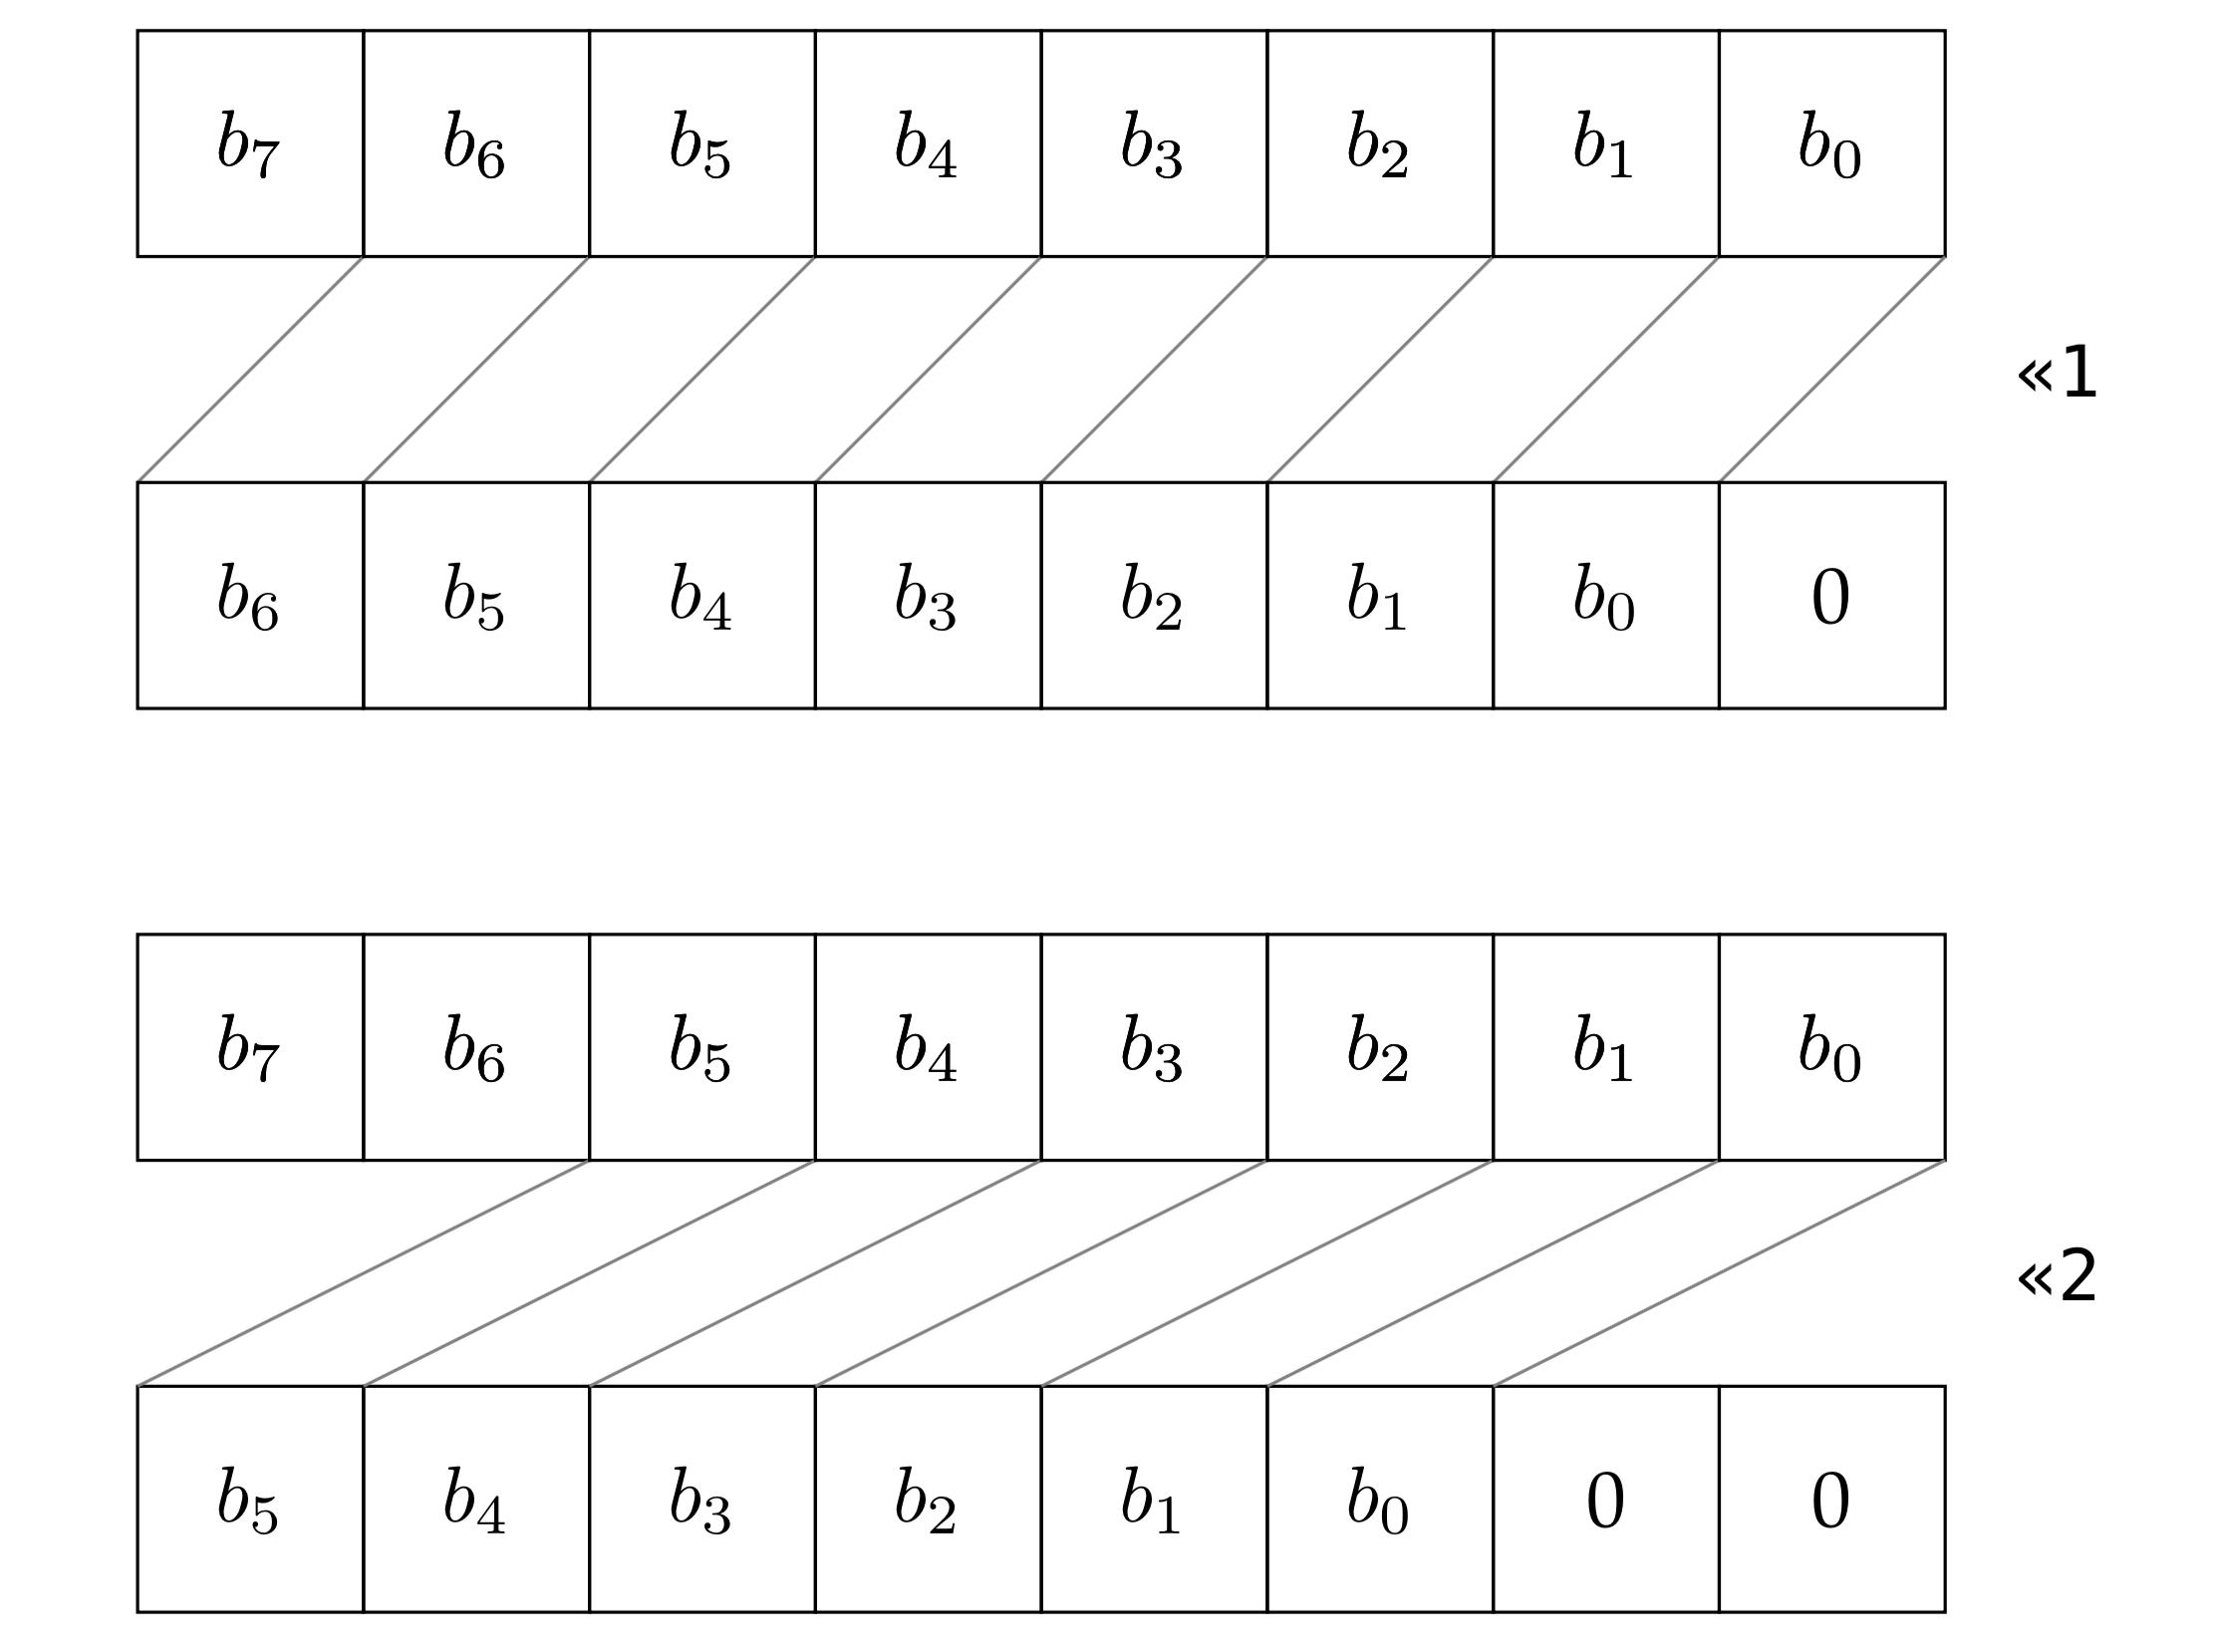
\includegraphics[width=0.8\textwidth]{img/left-shift.png}
\end{center}
%%%% TIKZ picture for image above
%% $$
%% \begin{tikzpicture}
%%   \foreach \i in {0,1,...,7}
%%   {
%%     \draw (\i,0) rectangle +(1,1);
%%     \node at (7-\i+0.5,0.5) {$b_\i$};
%%     \draw[gray] (\i+1,0) -- (\i,-1);
%%     \draw (\i,-2) rectangle +(1,1);
%%     \node at (7-\i+0.5,0.5) {$b_\i$};
%% %    \ifthenelse{\i<7}{\node at (6-\i+0.5,-1.5) {$b_\i$};}{}
%%     \ifnumless{\i}{7}{\node at (6-\i+0.5,-1.5) {$b_\i$};}{}
%%   }
%%   \node at (7.5,-1.5) {0};
%%   \node at (8.5,-0.5) {\texttt{<<1}}; % >>
%%   \begin{scope}[yshift=-4cm]
%%   \foreach \i in {0,1,...,7}
%%   {
%%     \draw (\i,0) rectangle +(1,1);
%%     \node at (7-\i+0.5,0.5) {$b_\i$};
%% %    \ifthenelse{\i>0}{\draw[gray] (\i+1,0) -- (\i-1,-1);}{}
%%      \ifnumgreater{\i}{0}{\draw[gray] (\i+1,0) -- (\i-1,-1);}{}
%%     \draw (\i,-2) rectangle +(1,1);
%%     \node at (7-\i+0.5,0.5) {$b_\i$};
%% %    \ifthenelse{\i<6}{\node at (5-\i+0.5,-1.5) {$b_\i$};}{}
%%     \ifnumless{\i}{6}{\node at (5-\i+0.5,-1.5) {$b_\i$};}{}
%%   }
%%   \node at (7.5,-1.5) {0};
%%   \node at (6.5,-1.5) {0};
%%   \node at (8.5,-0.5) {\texttt{<<2}}; % >>
%%   \end{scope}
%% \end{tikzpicture}
%% $$
\end{gram}

\begin{gram}
The right shift, \lstinline'x >> k' (for $0 \leq k < 32$), copies the
highest bit while shifting to the right, so that bits $31, \ldots,
32-k$ of the result will be equal to the highest bit of $x$.
If viewing $x$ as an integer, this means that the sign of the result
is equal to the sign of $x$, and shifting $x$ right by $k$ bits
corresponds to integer division by $2^k$ except that it truncates
towards $-\infty$.  For example, \lstinline'-1 >> 1 == -1'.

\begin{center}
  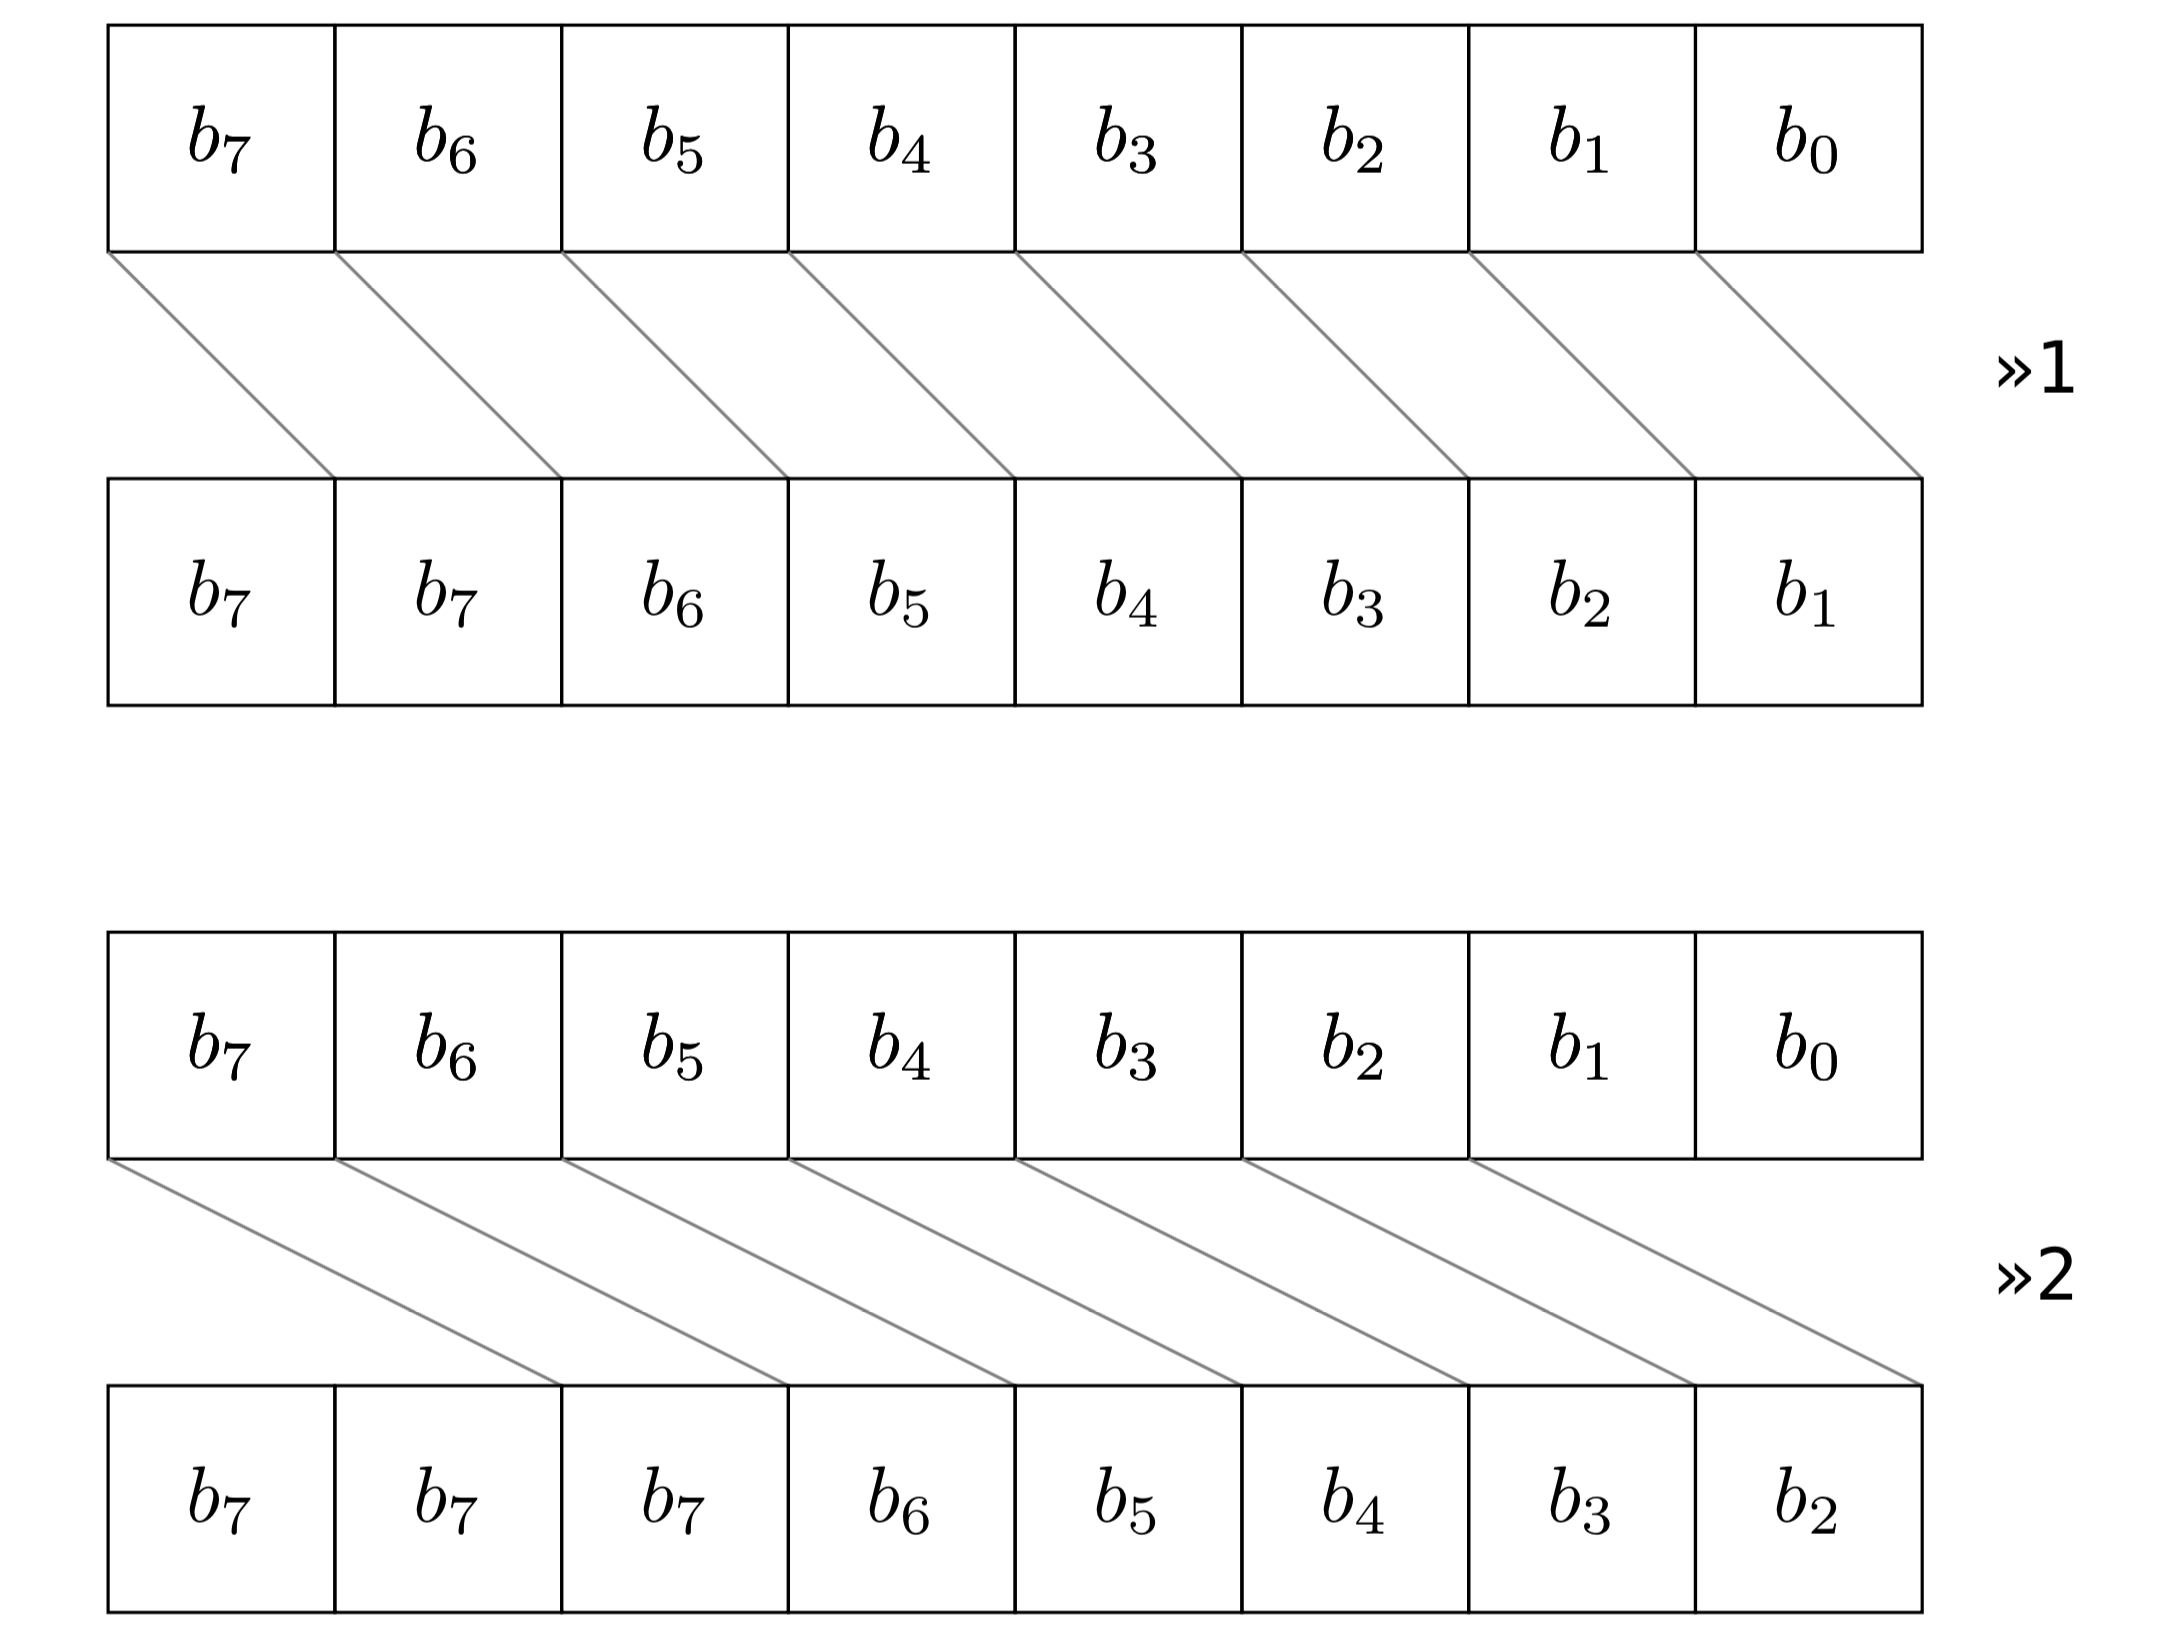
\includegraphics[width=0.8\textwidth]{img/right-shift.png}
\end{center}
%%% TIKZ picture of image above
%% $$
%% \begin{tikzpicture}
%%   \foreach \i in {0,1,...,7}
%%   {
%%     \draw (\i,0) rectangle +(1,1);
%%     \node at (7-\i+0.5,0.5) {$b_\i$};
%%     \draw[gray] (\i,0) -- (\i+1,-1);
%%     \draw (\i,-2) rectangle +(1,1);
%%     \node at (7-\i+0.5,0.5) {$b_\i$};
%% %    \ifthenelse{\i>0}{\node at (8-\i+0.5,-1.5) {$b_\i$};}{}
%%     \ifnumgreater{\i}{0}{\node at (8-\i+0.5,-1.5) {$b_\i$};}{}
%%   }
%%   \node at (0.5,-1.5) {$b_7$};
%%   \node at (8.5,-0.5) {\texttt{>>1}};
%%   \begin{scope}[yshift=-4cm]
%%   \foreach \i in {0,1,...,7}
%%   {
%%     \draw (\i,0) rectangle +(1,1);
%%     \node at (7-\i+0.5,0.5) {$b_\i$};
%% %    \ifthenelse{\i<7}{\draw[gray] (\i,0) -- (\i+2,-1);}{}
%%     \ifnumless{\i}{7}{\draw[gray] (\i,0) -- (\i+2,-1);}{}
%%     \draw (\i,-2) rectangle +(1,1);
%%     \node at (7-\i+0.5,0.5) {$b_\i$};
%% %    \ifthenelse{\i>1}{\node at (9-\i+0.5,-1.5) {$b_\i$};}{}
%%     \ifnumgreater{\i}{1}{\node at (9-\i+0.5,-1.5) {$b_\i$};}{}
%%   }
%%   \node at (0.5,-1.5) {$b_7$};
%%   \node at (1.5,-1.5) {$b_7$};
%%   \node at (8.5,-0.5) {\texttt{>>2}};
%%   \end{scope}
%% \end{tikzpicture}
%% $$
\end{gram}

\section{Representing Colors}
\label{sec:ints:colors}
\TAGS{application, ints, bit-patterns}

As a small example of using the bitwise interpretation of
\lstinline'int's, we consider colors.  Colors are decomposed into
their primary components red, green, and blue; the intensity of each
uses 8 bits and therefore varies between $0$ and $255$ (or
\lstinline'0x00' and \lstinline'0xFF').  We also have the so-called
\emph{$\alpha$-channel} which indicates how opaque the color is when
superimposed over its background.  Here, \lstinline'0xFF' indicates
completely opaque, and \lstinline'0x00' completely transparent.

\begin{example}
For example, to extract the intensity of the red color in a given
pixel $p$, we could compute \lstinline'(p >> 16) & 0xFF'.  The first shift
moves the red color value into the bits $0$--$7$; the bitwise and
masks out all the other bits by setting them to $0$.  The result will
always be in the desired range, from $0$--$255$.

Conversely, if we want to set the intensity of green of the pixel $p$
to the value of $g$ (assuming we already have $0 \leq g \leq 255$), we
can compute \lstinline'(p & 0xFFFF00FF) | (g << 8)'.  This works by first
setting the green intensity to $0$, while keep everything else the same,
and then combining it with the value of $g$, shifted to the right
position in the word.

For more on color values and some examples, see Assignment 1.
\end{example}

\clearpage
\section{Exercises}
\label{sec:ints:exercises}

\begin{exercise}\label{ex:ints:quotrem}
  Write functions \lstinline'quot' and \lstinline'rem' that calculate quotient
  and remainder as explained in Section~\ref{sec:ints:div}.  Your functions
  should have the property that
\begin{lstlisting}[language={[C0]C}]
quot(x,y)*y + rem(x,y) == x;
\end{lstlisting}
for all \lstinline'int's $x$ and $y$ unless \lstinline'quot'
overflows.  How is that possible?
\end{exercise}

\begin{exercise}
  Write a function \lstinline'int2hex' that returns a string containing the
  hexadecimal representation of a given integer as a string.  Your
  function should have prototype
\begin{lstlisting}[language={[C0]C}]
string int2hex(int x);
\end{lstlisting}
(The \emph{prototype} of a function is the function without its body:
the prototype gives the function name and the type of its arguments.)
\end{exercise}


\begin{exercise}
  Write a function \lstinline'lsr' (logical shift right), which is like
  right shift (\lstinline'>>') except that it fills the most significant
  bits with zeroes instead of copying the sign bit.  Explain what
  \lstinline'lsr(x,1)' means on integers in two's complement
  representation.
\end{exercise}


\begin{flex}
\begin{exercise}%[\opt{sample solution on page~\pageref{ex:fast_pow-overflow-solved}}]
\label{ex:fast_pow-overflow}
\exerciseTAGS{ints, safety}
  Rewrite the functions \lstinline'POW' and \lstinline'f' (the mystery
  function) from Chapter~\ref{ch:contracts} so that they signal an
  error in case of an overflow rather than silently working in modular
  arithmetic.  You can use the statement
  \lstinline'error("Overflow");' to signal an overflow. Don't worry about
  catching overflow with a negative base --- that's a little more
  complicated.
\end{exercise}

\begin{solution}\opt{\textbf{of exercise~\ref{ex:fast_pow-overflow}}}
\label{ex:fast_pow-overflow-solved}
\begin{lstlisting}[language={[C0]C}]
int POW (int x, int y)
//@requires y >= 0;
{
  if (y == 0)
    return 1;
  int p = x * POW(x, y-1);
  if (x > 0 && p <= 0)  error("Overflow");
  return p;
}
\end{lstlisting}
If what gets returned from a recursive call is ever negative, we know
for sure we have had an overflow.  This holds also if this value is
0, but only if \lstinline'x' did not start at 0.

\begin{lstlisting}[language={[C0]C}]
int f(int x, int y)
//@requires y >= 0;
//@ensures \result == POW(x,y);
{
  int r = 1;
  int b = x;           /* base     */
  int e = y;           /* exponent */
  while (e > 0)
  //@loop_invariant e >= 0;
  //@loop_invariant r * POW(b,e) == POW(x,y);
  {
    if (e % 2 == 1) {
      r = b * r;
      if (x > 0 && r <= 0) error("Overflow");
    }
    b = b * b;
    e = e / 2;
  }
  //@assert e == 0;
  return r;
}
\end{lstlisting}
Putting a similar check after \lstinline'b = b*b' would be incorrect:
performing this computation on the last iteration (when
\lstinline'e==1') does not influence the result of the function and
therefore it is unimportant whether it overflows.

Note that this isn't how we'd normally want to detect overflow.
We'll talk about this later in the course, but we'd rather
notice that overflow will happen before actually causing it,
rather than noticing after it happens.
\end{solution}
\end{flex}


\printsolutions
% \clearpage
% \bibliographystyle{alpha}
% \bibliography{modal}
